\chapter{\label{ch:1-intro}Introduction} 

\graphicspath{{figures/ch1/}}

\minitoc

\section{General introduction}

\section{Structure and function of the pancreatic K\textsubscript{ATP} channel}

\subsection{Pancreatic islets and the \textgreek{b}-cell}

Pancreatic islets are endocrine cells which are responsible for maintaining glucose homeostasis.
There are roughly one million islets in a human pancreas, constituting 1-2\% of the total pancreatic mass.
Islets consist of three principal cell types; insulin secreting \textgreek{b}-cells, glucagon secreting \textgreek{a}-cells and somatostatin secreting \textgreek{d}-cells.
Islets respond to increases in blood glucose by releasing insulin, which acts on peripheral tissues to increase glucose uptake and reduce blood glucose levels.
Conversely, decreases in blood glucose leads to the release of glucagon, which acts on those tissues to stimulate glucose production and increase blood glucose.

\subsection{Glucose induced insulin secretion in \textgreek{b}-cells}

\subsection{Architecture of the pancreatic K\textsubscript{ATP} channel}

ATP-sensitive potassium (K\textsubscript{ATP}) channels are present in many tissues, where they couple the metabolic state of a cell to its electrical activity by regulating the flow of K\textsuperscript{+} across the membrane.
K\textsubscript{ATP} channels are an octameric complex, comprised of four inwardly-rectifying potassium channel subunits (Kir6.1 or Kir6.2), each of which is associated with a sulphonylurea receptor subunit (SUR1, SUR2A or SUR2B).
In pancreatic \textgreek{b}-cells, the K\textsubscript{ATP} channel isoform is composed of Kir6.2 and SUR1.

Inwardly-rectifying potassium channels are so named because they allow K\textsuperscript{+} to flow more easily into the cell than out of it.
This phenomenon is a consequence of voltage-dependent pore blockade by intracellular divalent cations (especially Mg\textsuperscript{2+}) and polyamines.
At depolarising membrane potentials, blockers are driven into the pore and K\textsuperscript{+} current is blocked, while at hyperpolarising potentials the blockers and cleared and K\textsuperscript{+} current can flow.
Strongly rectifying Kir channels display drastically reduced conductance at potentials more positive than the K\textsuperscript{+} reversal potential.
In contrast, Kir6.2 is a weak rectifier, and allows substantial current to flow at more positive potentials.

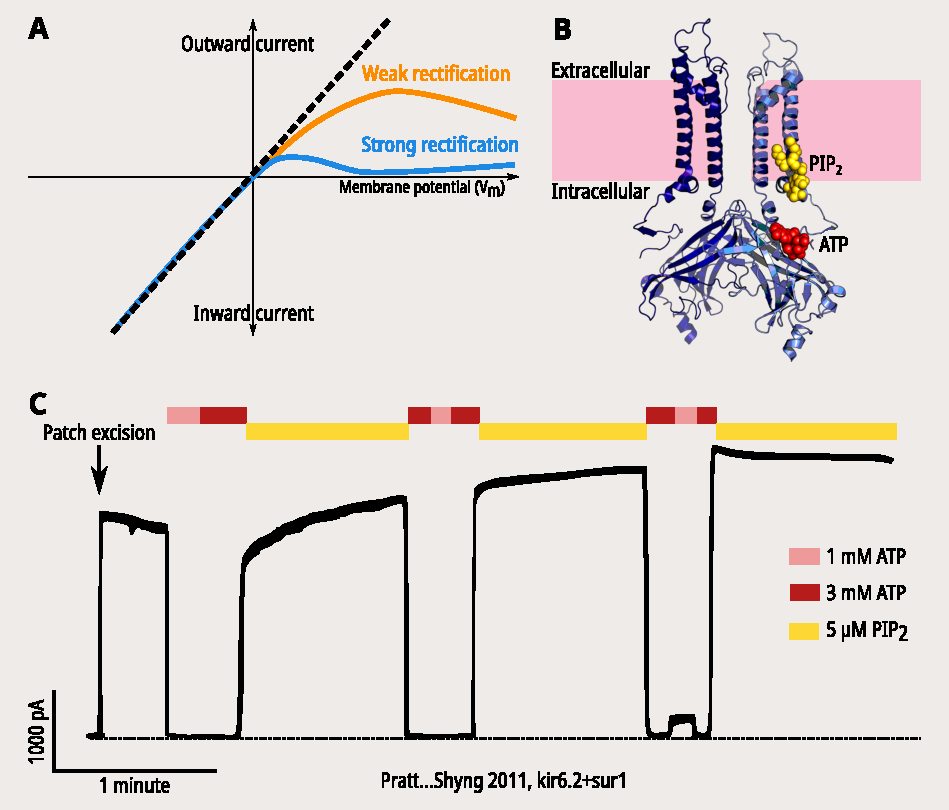
\includegraphics[width=0.9\textwidth]{rectification.pdf}

In addition to voltage, Kir6.2 is regulated by two endogenous ligands; 
phosphatidylinositol 4,5-bisphosphate (PIP\textsubscript{2}) and adenine nucleotides (ATP/ADP).
The binding of adenine nucleotides to Kir6.2 leads to closure of the channel pore, while the binding of PIP2 promotes the opening of the pore.


\subsection{Nucleotide regulation of the pancreatic K\textsubscript{ATP} channel}

\section{Fluorescence methods in ion channel research}

\subsection{Fluorescence as a tool}

\subsection{Forster resonance energy transfer}

\subsection{Unnatural amino acid incorporation}

\section{Functional modelling of ion channels}

\subsection{Why?}

\subsection{A model that fits}
